\subsection{Advantage}
Una vez demostrada la relevancia, nos planteamos que beneficios y ventajas que nos puede traer la utilizacion de los datos como usuario. 
Este objetivo requiere de trabajo minucioso tanto para descubrirlo como para transmitir estos conceptos al usuario de forma clara, 
sencilla y directa y asi lograr un vinculo que haga crecer la curiosidad del usuario de profundizar en la materia y
mantenerse informado.

Es muy importante pornerse en el lugar del usuario y descubrir que es realmente necesario para el. Solo si el usuario entiende la relevancia de 
los datos y la influencia que estos tienen en su vida diaria, sera posible un compromiso por parte de este.

Es decir, la informacion debera cubrir una necesidad del usuario, aunque el usuario no sepa a priori que tiene esta necesidad. Quizas sea 
nuestro objetivo dejarle ver lo util y ventajoso que puede ser la utilizacion de estos datos.

Cuando tengamos unos datos que se actualizen periodicamente, deberemos de pensar en que manera puedan interesarnos las fluctuacion o que ciertos
cambios. Aqui entra en juego la representacion de la informacion de una manera que despierte la necesidad de monitorizacion de los datos por parte
del usuario.

\subsubsection{How to solve it} 
En primer lugar descubrir de que manera los datos pueden ayudar a los usuarios. A continuacion se ha de buscar la manera de dejarle ver
porque son importantes para el y como puede beneficiar el uso de ellos en su vida diaria.
Si los datos se actualizan periodicamente, hay que analizar que tipo de variaciones son importantes en la vida cotidiana del usuario.
Realizar un estudio de mercado y ver si ya existen productos que ofrezcan esta informacion. Si este es el caso, se analizara porque no
resulta atractiva al usuario e intentar mejorarlo.

\subsubsection{How we solve it. Aire Guru} 
Se le ofrece al usuario una plataforma que le indica su exposicion a la polucion del aire totalmente personalizada si la necesidad de acarrear
ningun dispositivo para la lectura de los contaminantes.



Aire Guru previo permiso explicito de lectura de la localizacion por parte del usuario, recoge el poligono donde
se encuentra el usuario y almacena la medida de la polucion mas reciente para ese poligono. A continuacion, el 
usuario podra visualizar la exposicion a la contaminacion a la que ha sido sometido.

\begin{figure}[ht]
    \centering 
    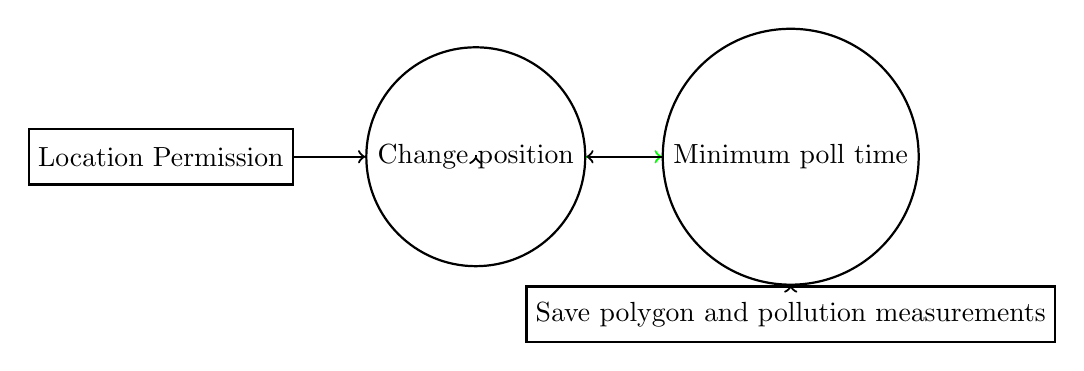
\begin{tikzpicture}[thick]
        \node[draw,rectangle,minimum size=20] (a) {Location Permission};
         \node[draw,circle,minimum size=6,right of= a, node distance=4cm] (b) {Change position};
         \node[draw,circle,minimum size=5,right of= b, node distance=4cm] (c) {Minimum poll time};
         \node[draw,rectangle,minimum size=20,below of=c, node distance=2cm] (d) {Save polygon and pollution measurements};
         \draw[->] (a) to (b);
         \draw[->] (b) to (b);
        \draw[->,green] (b) to (c);
        \draw[->] (c) to (d);
     \draw[->] (c) to (b);
      \end{tikzpicture}
      \caption{Collecting user location}
    \end{figure}
    \newpage
    \begin{figure}[ht]
        \centering
        \includegraphics[width=8cm]{importedDataDecember}
        \caption{Personal Records. December}
    \end{figure}

Se puede ver la exposicion a la polucion del aire desde el 2018 sin tener que haber estado usando la herramienta ya que
mediante el boton importar cronologia de Google, se puede importar el historial de localizacion que proporcionara la
contaminacion a la que se ha estado expuesto desde el 2018. En la seccion de ayuda podemos encontrar una guia de como se 
exportar e importa este historial de localizaciones.
\begin{comment}
    

\begin{figure}[ht]
    \centering
    \includegraphics[width=11cm]{helpImport}
    \caption{First step Import Google Location}
\end{figure}
\end{comment}
\elsparagraph{Evaluation}  
\begin{itemize}
    \done Caracteristica unica, monitorizacion de la exposicion de la polucion completamente personalizada
    \done Descripcion de los efectos, fuentes contaminantes, descripcion de los contaminantes en una unica plataforma
    \crossed Presentar como se puede reducir la exposicion a la polucion mas especificamente
    
\end{itemize}
\newpage